%==============================================================================
% tento soubor pouzijte jako zaklad
% this file should be used as a base for the thesis
% Autoři / Authors: 2008 Michal Bidlo, 2019 Jaroslav Dytrych
% Kontakt pro dotazy a připomínky: sablona@fit.vutbr.cz
% Contact for questions and comments: sablona@fit.vutbr.cz
%==============================================================================
% kodovani: UTF-8 (zmena prikazem iconv, recode nebo cstocs)
% encoding: UTF-8 (you can change it by command iconv, recode or cstocs)
%------------------------------------------------------------------------------
% zpracování / processing: make, make pdf, make clean
%==============================================================================
% Soubory, které je nutné upravit nebo smazat: / Files which have to be edited or deleted:
%   projekt-20-literatura-bibliography.bib - literatura / bibliography
%   projekt-01-kapitoly-chapters.tex - obsah práce / the thesis content
%   projekt-01-kapitoly-chapters-en.tex - obsah práce v angličtině / the thesis content in English
%   projekt-30-prilohy-appendices.tex - přílohy / appendices
%   projekt-30-prilohy-appendices-en.tex - přílohy v angličtině / appendices in English
%==============================================================================
\documentclass[slovak, zadani]{fitthesis} % bez zadání - pro začátek práce, aby nebyl problém s překladem
%\documentclass[english]{fitthesis} % without assignment - for the work start to avoid compilation problem
%\documentclass[zadani]{fitthesis} % odevzdani do wisu a/nebo tisk s barevnými odkazy - odkazy jsou barevné
%\documentclass[english,zadani]{fitthesis} % for submission to the IS FIT and/or print with color links - links are color
%\documentclass[zadani,print]{fitthesis} % pro černobílý tisk - odkazy jsou černé
%\documentclass[english,zadani,print]{fitthesis} % for the black and white print - links are black
%\documentclass[zadani,cprint]{fitthesis} % pro barevný tisk - odkazy jsou černé, znak VUT barevný
%\documentclass[english,zadani,cprint]{fitthesis} % for the print - links are black, logo is color
% * Je-li práce psaná v anglickém jazyce, je zapotřebí u třídy použít 
%   parametr english následovně:
%   If thesis is written in English, it is necessary to use 
%   parameter english as follows:
%      \documentclass[english]{fitthesis}
% * Je-li práce psaná ve slovenském jazyce, je zapotřebí u třídy použít 
%   parametr slovak následovně:
%   If the work is written in the Slovak language, it is necessary 
%   to use parameter slovak as follows:
%      \documentclass[slovak]{fitthesis}
% * Je-li práce psaná v anglickém jazyce se slovenským abstraktem apod., 
%   je zapotřebí u třídy použít parametry english a enslovak následovně:
%   If the work is written in English with the Slovak abstract, etc., 
%   it is necessary to use parameters english and enslovak as follows:
%      \documentclass[english,enslovak]{fitthesis}

% Základní balíčky jsou dole v souboru šablony fitthesis.cls
% Basic packages are at the bottom of template file fitthesis.cls
% zde můžeme vložit vlastní balíčky / you can place own packages here

% Kompilace po částech (rychlejší, ale v náhledu nemusí být vše aktuální)
% Compilation piecewise (faster, but not all parts in preview will be up-to-date)
% \usepackage{subfiles}

% Nastavení cesty k obrázkům
% Setting of a path to the pictures
%\graphicspath{{obrazky-figures/}{./obrazky-figures/}}
%\graphicspath{{obrazky-figures/}{../obrazky-figures/}}

%---rm---------------
\renewcommand{\rmdefault}{lmr}%zavede Latin Modern Roman jako rm / set Latin Modern Roman as rm
%---sf---------------
\renewcommand{\sfdefault}{qhv}%zavede TeX Gyre Heros jako sf
%---tt------------
\renewcommand{\ttdefault}{lmtt}% zavede Latin Modern tt jako tt

% vypne funkci šablony, která automaticky nahrazuje uvozovky,
% aby nebyly prováděny nevhodné náhrady v popisech API apod.
% disables function of the template which replaces quotation marks
% to avoid unnecessary replacements in the API descriptions etc.
\csdoublequotesoff



\usepackage{url}


% =======================================================================
% balíček "hyperref" vytváří klikací odkazy v pdf, pokud tedy použijeme pdflatex
% problém je, že balíček hyperref musí být uveden jako poslední, takže nemůže
% být v šabloně
% "hyperref" package create clickable links in pdf if you are using pdflatex.
% Problem is that this package have to be introduced as the last one so it 
% can not be placed in the template file.
\ifWis
\ifx\pdfoutput\undefined % nejedeme pod pdflatexem / we are not using pdflatex
\else
  \usepackage{color}
  \usepackage[unicode,colorlinks,hyperindex,plainpages=false,pdftex]{hyperref}
  \definecolor{hrcolor-ref}{RGB}{223,52,30}
  \definecolor{hrcolor-cite}{HTML}{2F8F00}
  \definecolor{hrcolor-urls}{HTML}{092EAB}
  \hypersetup{
	linkcolor=hrcolor-ref,
	citecolor=hrcolor-cite,
	filecolor=magenta,
	urlcolor=hrcolor-urls
  }
  \def\pdfBorderAttrs{/Border [0 0 0] }  % bez okrajů kolem odkazů / without margins around links
  \pdfcompresslevel=9
\fi
\else % pro tisk budou odkazy, na které se dá klikat, černé / for the print clickable links will be black
\ifx\pdfoutput\undefined % nejedeme pod pdflatexem / we are not using pdflatex
\else
  \usepackage{color}
  \usepackage[unicode,colorlinks,hyperindex,plainpages=false,pdftex,urlcolor=black,linkcolor=black,citecolor=black]{hyperref}
  \definecolor{links}{rgb}{0,0,0}
  \definecolor{anchors}{rgb}{0,0,0}
  \def\AnchorColor{anchors}
  \def\LinkColor{links}
  \def\pdfBorderAttrs{/Border [0 0 0] } % bez okrajů kolem odkazů / without margins around links
  \pdfcompresslevel=9
\fi
\fi
% Řešení problému, kdy klikací odkazy na obrázky vedou za obrázek
% This solves the problems with links which leads after the picture
\usepackage[all]{hypcap}

% Informace o práci/projektu / Information about the thesis
%---------------------------------------------------------------------------
\projectinfo{
  %Prace / Thesis
  project={BP},            %typ práce BP/SP/DP/DR  / thesis type (SP = term project)
  year={2020},             % rok odevzdání / year of submission
  date=\today,             % datum odevzdání / submission date
  %Nazev prace / thesis title
  title.cs={Generování sekvenčních diagramů z modelů Petriho sítí},  % název práce v češtině či slovenštině (dle zadání) / thesis title in czech language (according to assignment)
  title.en={Code Generation from Object Oriented Petri Nets}, % název práce v angličtině / thesis title in english
  %title.length={14.5cm}, % nastavení délky bloku s titulkem pro úpravu zalomení řádku (lze definovat zde nebo níže) / setting the length of a block with a thesis title for adjusting a line break (can be defined here or below)
  %sectitle.length={14.5cm}, % nastavení délky bloku s druhým titulkem pro úpravu zalomení řádku (lze definovat zde nebo níže) / setting the length of a block with a second thesis title for adjusting a line break (can be defined here or below)
  %Autor / Author
  author.name={Erik},   % jméno autora / author name
  author.surname={Kelemen},   % příjmení autora / author surname 
  %author.title.p={Bc.}, % titul před jménem (nepovinné) / title before the name (optional)
  %author.title.a={Ph.D.}, % titul za jménem (nepovinné) / title after the name (optional)
  %Ustav / Department
  department={UITS}, % doplňte příslušnou zkratku dle ústavu na zadání: UPSY/UIFS/UITS/UPGM / fill in appropriate abbreviation of the department according to assignment: UPSY/UIFS/UITS/UPGM
  % Školitel / supervisor
  supervisor.name={Radek},   % jméno školitele / supervisor name 
  supervisor.surname={Kočí},   % příjmení školitele / supervisor surname
  supervisor.title.p={Ing.},   %titul před jménem (nepovinné) / title before the name (optional)
  supervisor.title.a={Ph.D.},    %titul za jménem (nepovinné) / title after the name (optional)
  % Klíčová slova / keywords
  keywords.cs={objektovo orientované petriho siete, sekvenčný diagram, simulácia.}, % klíčová slova v českém či slovenském jazyce / keywords in czech or slovak language
  keywords.en={object oriented petri nets, sequence diagram, simulation}, % klíčová slova v anglickém jazyce / keywords in english
  %keywords.en={Here, individual keywords separated by commas will be written in English.},
  % Abstrakt / Abstract
  abstract.cs={Zatiaľ čo petriho siete nesporne dominujú v monitorovaní zmeny stavov v modelovanom systéme, sekvenčné diagramy dokážu lepšie prezentovať externý pohľad na systém v časovom slede posielaných správ medzi objektami podieľajúcimi sa na komunikácii. I keď by sa mohlo zdať, že majú spolu pramálo spoločného, v tejto práci bude predvedeny koncept ako vygenerovať sekvenčný diagram pomocou simulácie modelu objektovo orientovanej petriho siete zapísaného v jazyku PNTalk bez dodatočných informácií, ktoré by akokoľvek pomohli zostaviť sekvenčný diagram. Práca sa zaoberá transformáciou dát v zmysle minimálnej straty informácie z modelu objektovo orientovaných peteriho sietí a následnú prezentáciu vyťažených dát a to nad rámec triviálnych sekvenčných diagramov. }, % abstrakt v českém či slovenském jazyce / abstract in czech or slovak language
  abstract.en={Do tohoto odstavce bude zapsán výtah (abstrakt) práce v anglickém jazyce.}, % abstrakt v anglickém jazyce / abstract in english
  %abstract.en={An abstract of the work in English will be written in this paragraph.},
  % Prohlášení (u anglicky psané práce anglicky, u slovensky psané práce slovensky) / Declaration (for thesis in english should be in english)
  declaration={Prehlasujem, že som túto bakalársku prácu vypracoval samostatne pod vedením pána Radek Kočí.
Další informace mi poskytli Tomáš Lapšanský ako konzultant práce na ktorú som priamo nadviazal.
Uvedl jsem všechny literární prameny, publikace a další zdroje, ze kterých jsem čerpal.},
  %declaration={I hereby declare that this Bachelor's thesis was prepared as an original work by the author under the supervision of Mr. X
% The supplementary information was provided by Mr. Y
% I have listed all the literary sources, publications and other sources, which were used during the preparation of this thesis.},
  % Poděkování (nepovinné, nejlépe v jazyce práce) / Acknowledgement (optional, ideally in the language of the thesis)
  acknowledgment={V této sekci je možno uvést poděkování vedoucímu práce a těm, kteří poskytli odbornou pomoc
(externí zadavatel, konzultant apod.).},
  %acknowledgment={Here it is possible to express thanks to the supervisor and to the people which provided professional help
%(external submitter, consultant, etc.).},
  % Rozšířený abstrakt (cca 3 normostrany) - lze definovat zde nebo níže / Extended abstract (approximately 3 standard pages) - can be defined here or below
  %extendedabstract={Do tohoto odstavce bude zapsán rozšířený výtah (abstrakt) práce v českém (slovenském) jazyce.},
  %faculty={FIT}, % FIT/FEKT/FSI/FA/FCH/FP/FAST/FAVU/USI/DEF
  faculty.cs={Fakulta informačních technologií}, % Fakulta v češtině - pro využití této položky výše zvolte fakultu DEF / Faculty in Czech - for use of this entry select DEF above
  faculty.en={Faculty of Information Technology}, % Fakulta v angličtině - pro využití této položky výše zvolte fakultu DEF / Faculty in English - for use of this entry select DEF above
  department.cs={Ústav matematiky}, % Ústav v češtině - pro využití této položky výše zvolte ústav DEF nebo jej zakomentujte / Department in Czech - for use of this entry select DEF above or comment it out
  department.en={Institute of Mathematics} % Ústav v angličtině - pro využití této položky výše zvolte ústav DEF nebo jej zakomentujte / Department in English - for use of this entry select DEF above or comment it out
}

% Rozšířený abstrakt (cca 3 normostrany) - lze definovat zde nebo výše / Extended abstract (approximately 3 standard pages) - can be defined here or above
%\extendedabstract{Do tohoto odstavce bude zapsán výtah (abstrakt) práce v českém (slovenském) jazyce.}

% nastavení délky bloku s titulkem pro úpravu zalomení řádku - lze definovat zde nebo výše / setting the length of a block with a thesis title for adjusting a line break - can be defined here or above
%\titlelength{14.5cm}
% nastavení délky bloku s druhým titulkem pro úpravu zalomení řádku - lze definovat zde nebo výše / setting the length of a block with a second thesis title for adjusting a line break - can be defined here or above
%\sectitlelength{14.5cm}

% řeší první/poslední řádek odstavce na předchozí/následující stránce
% solves first/last row of the paragraph on the previous/next page
\clubpenalty=10000
\widowpenalty=10000

% checklist
\newlist{checklist}{itemize}{1}
\setlist[checklist]{label=$\square$}

\begin{document}
  % Vysazeni titulnich stran / Typesetting of the title pages
  % ----------------------------------------------
  \maketitle
  %\includepdf[pages=-, offset= 0cm -3.54cm]{zadanie.pdf}
  % Obsah
  % ----------------------------------------------
  \setlength{\parskip}{0pt}

  {\hypersetup{hidelinks}\tableofcontents}
  
  % Seznam obrazku a tabulek (pokud prace obsahuje velke mnozstvi obrazku, tak se to hodi)
  % List of figures and list of tables (if the thesis contains a lot of pictures, it is good)
  \ifczech
    \renewcommand\listfigurename{Seznam obrázků}
  \fi
  \ifslovak
    \renewcommand\listfigurename{Zoznam obrázkov}
  \fi
  % {\hypersetup{hidelinks}\listoffigures}
  
  \ifczech
    \renewcommand\listtablename{Seznam tabulek}
  \fi
  \ifslovak
    \renewcommand\listtablename{Zoznam tabuliek}
  \fi
  % {\hypersetup{hidelinks}\listoftables}

  \ifODSAZ
    \setlength{\parskip}{0.5\bigskipamount}
  \else
    \setlength{\parskip}{0pt}
  \fi

  % vynechani stranky v oboustrannem rezimu
  % Skip the page in the two-sided mode
  \iftwoside
    \cleardoublepage
  \fi

  % Text prace / Thesis text
  % ----------------------------------------------
  \ifenglish
    \input{projekt-01-kapitoly-chapters-en}
  \else
    \theoremstyle{definition}
\newtheorem{defn}{Definícia}[section]
\newtheorem{note}{Poznámka}[section]
\newtheorem{exmpl}{Príklad}[section]

\chapter{Úvod}


Jeden z najzákladnejších problémov, ktoré rieši softvérový vývoj je validácia požiadavkov systému. Tieto požiadavky sú zvyčajne definované pomocou diagramu užitia z UML. 
Bežný postup je navrhnúť model systému podľa týchto požiadaviek za pomoci ostatných diagramov z UML a otestovať ho manuálne implementovaným prototypom. To predstavuje dosť práce jednak s diagramami UML a navyše implementovaný prototyp pravdepodobne stratí veškeré využitie po validácii modelu. Predstavme si však, že vytvoríme model za použitia objektovo orientovaných petriho sietí, ktorý prichádza s možnosťou simulácie modelu. Táto simulácia poskytuje priestor na automatické vytvorenie UML diagramov. Isteže existujú aj rozšírenia UML a metódy na ich prevod do spustiteľnej formy ako MDA methodology, Executable UML (xUML) language alebo Foundational Subset pre xUML, všetky zo zmienených metód však trpia nedostatkom, keď sa spustitelná forma UML modelu v priebehu validácie upravuje, je takmer nemožné vrátiť sa so zmenamy k pôvodnému modelu. 

Hlavným cieľom práce je vytvoriť plnohodnotný nástroj na validáciu modelu, ktorý vygeneruje sekvenčný diagram z jazyka UML. Jazyk UML definuje viac diagramov interakcií z ktorých by sa dalo vybrať, no narozdiel od diagramu interakcií sa dá vygenerovať zo simulácie a navyše je sekvenčný diagram druhý nanajvýš používaný z diagramov UML. Od nástroja sa očakáva, že by mal analyzovať všetky možné scenáre, rozlíšiť redundantné výskyty častí scenárov a agregovať ich, aby obmedzil zobrazované informácie. Ďalej by mal poskytovať intuitívne rozhranie a zachovať všetky informácie zo simulácie ľahko dohľadateľné.

Najzložitejšiu časť generovania sekvenčného diagramu predstavuje nahradzovanie dát potrebných na zostavenie sekvenčného diagramu, chýbajúcich v reprezentácii pomocou objektovo orientovaných petriho sietí.

V kapitole.. TODO

\chapter{Úvod2}

Jeden z najzákladnejších problémov, ktoré rieši softvérový vývoj v ranných fázach je modelovanie systému. K jednej zo zaužívaných variant pre modelovanie systému patrí jazyk UML (Unified Modeling Language) ku ktorému od roku 1997(štandart v1.1) patrí sekvenčný diagram ako jeden z diagramov na modelovanie interakcií v systéme. Na druhej strane máme Petriho siete(PT), matematický model, ktorý je schopný vyjadriť kauzalitu udalostí, asynchrónnost, paralelizmus a synchronizáciu. Petriho siete sa do UML dostali len ako inšpirácia pre diagram aktivít v roku 1999(v 1.3). Na prvý pohľad je zrejmé, že diagram interakcií s matematickým modelom Petriho sietí má pramálo spoločného a táto absencia relevantných informácii zrejme neumožňuje automatické generovanie z jedného modelu na druhý. 

To sa zmení pri transformácii PT Petriho sietí do  funkcionálnych Petriho sietí (FPN) a následnou transformáciou do objektovo orientovaných Petriho sietí (OOPN). Týmto prechodom sa priblížia invokačné prechody z funkcionálnych Petriho sietí k volaniam správ ako ich poznáme zo sekvenčných diagramov. Triedy OOPN sa priblížia k objektom sekvenčných diagramov. Táto analógia je základným stavebným kameňom pre vytvorenie funkčného generátoru sekvenčných diagramov z objektovo orientovaných Petriho sietí. Celá myšlienka pochádza z vedecko publicistického článku :TODO: reference 

Cieľom práce je okolo tejto myšlienky postaviť generátor, ktorého vstupom je kód jazyka PNTalk popisujúci OOPN a výstupom sekvenčný diagram. Na záver sa správnosť vygenerovaných diagramov posúdi v porovnaní s diagramami vytvorenými ručne odborníkami z praxe.

\chapter{Tvorba a analýza scenárov v modelovaní systému}

\section{Vývoj systému}

Pred ponorením sa do analýzy a modelovania softvéru, je nutno zmieniť, kde majú pri vývoji softvéru svoje miesto a aké aspekty ich ovplyvňujú.

\subsection{Zúčastnená strana}

Všetky fyzické osoby ovplyvňujúce vývoj softvéru môžme pre akýkoľvek systém klasifikovať do 5 skupín. Zobrazené sú na ľavej strane Obr. \ref{fig:system-inputs}. Podstatné je, že každá zo skupín má na systém iný uhol pohľadu.

\begin{enumerate}
	\item \textbf{Systémový analytici a projektový manažéri} sú špecialistami na analýzu a modelovanie, poskytujú ostatným skupinám poradenstvo a sú akýmsi mostom pri akomkoľvek komunikačnom šume vznikajúcom napríklad medzi menej technicky zdatnými majiteľmi a projektu a vývojármi.
	\item \textbf{Vývojári}, ktorý majú za úlohu celý systém zkonštruovať podľa návrhu softvérového dizajnéra riešia hlavne detaily implementácie. V menších firmách sú dizajnéry a vývojáry tí istí ľudia, no vo väčších sú tieto úlohy často oddelené.
	\item \textbf{Dizajnéri} zodpovedný za modelovanie architektúry systému z ich uhlu pohľadu riešia správnu voľbu technológie pre systém. Tendenciou je mať špecializovaného návrhára pre každú časť zvlášť, preto do tejto skupiny patria databázový administrátori, sieťový architekti, bezpečnostný experti a mnohí ďaľší.
	\item \textbf{Uživateľia} systému, sú v dnešnej dobe čím ďaľej technicky vyspelí a ďaľšou ich nespornou výhodou je počet, ktorý väčšinou prevyšuje ostatné skupiny. Z ich pohľadu na systém je najdôležitejšia funkcionalita, intuitívnosť používania a o cenu, či profit, narozdiel od majiteľov, nedbajú.
	\item \textbf{Majitelia} projektu, ktorých môže byť viac než jeden väčšinou riešia projekt z pohľadu financií. Na koľko ich to vyjde, aký bude profit, či benefity.
\end{enumerate}
\begin{figure}[H]
	\centering
	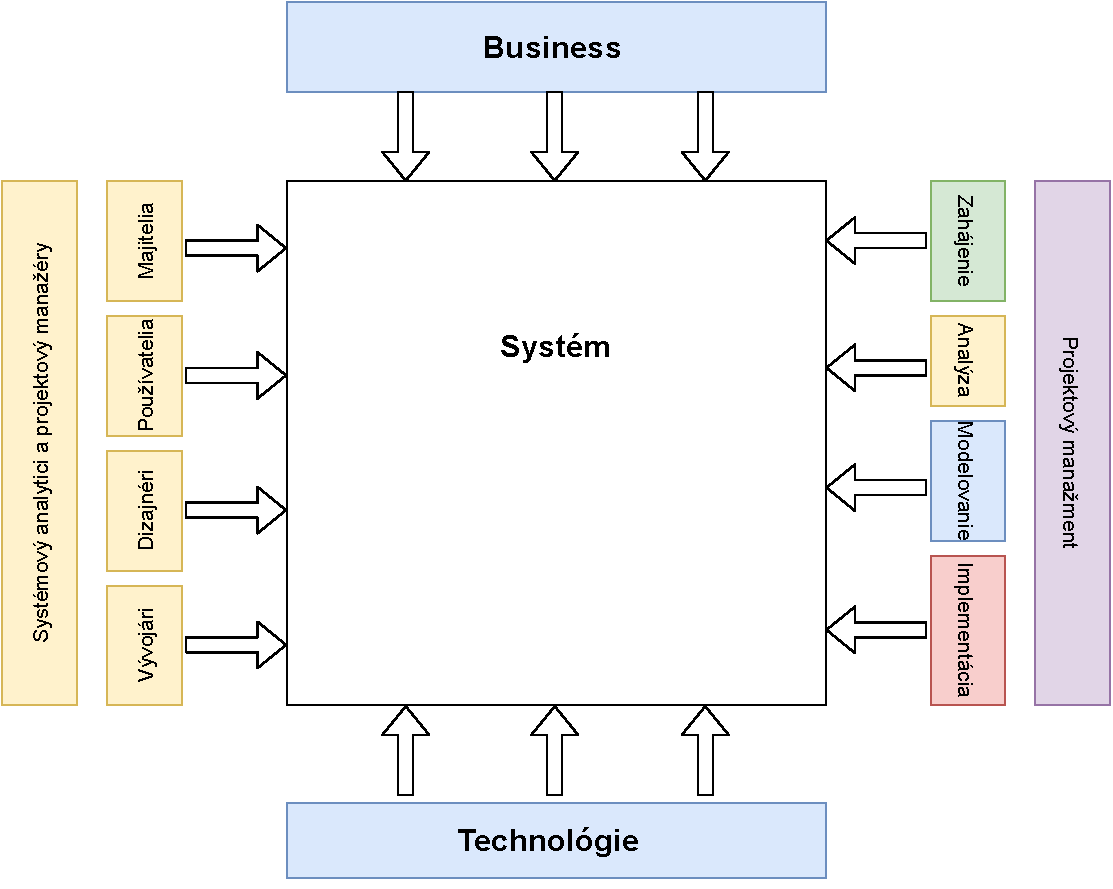
\includegraphics[scale=0.75]{obrazky-figures/TR-system-inputs}
	\caption{Aspekty ovplyvňujúce vývoj systému \cite{whitten2007systems}}
	\label{fig:system-inputs}
\end{figure}

\subsection{Iné factory}
Okrem Účastníkov vývoja majú na systém vplyv ešte aspekty businessu a technológie dostupné v dobe vývoja. Business pokrýva hlavne požiadavky obchodu spojené s legislatívou. Technológie nás obmedzujú pri nedostupnosti tak pokročilých technológií aké by sme potrebovali pre svoj systém alebo naopak nové prielomy v technológii poskytujú príležitosť pozdvihnnúť projekt na vyššiu úroveň.

\subsection{Procces vývoja}

Je zrejmé že väčšina organizácií bude mať vlastný formálne definovaný proces vývoja softvéru alebo sadu krokov, ktoré podľa ktorých by sa mal systém vyvíjať. Akiste sa budú tieto metodológie od seba diametrálne odlišovať pre jednotlivé organizácie. Avšak, všetky metódy riešenia problému môžeme zavšeobecniť na kroky, ktoré sú spoločné: \\

\begin{enumerate}
	\item \textbf{Identifikovať problém}, akokoľvek jednoducho prvý krok môže znieť opak je pravdou. Zadania sú často nejasné a ciele systému preto nejednoznačné. Rozsah práce môže byť podcenený s čím ide ruka v ruke aj časový plán a rozpočet.
	\item \textbf{Analyzovať a porozumieť problému}. Druhý krok poskytuje projektovému tímu hlbšie porozumenie systému, vyžaduje spoluprácu so zúčastnenou stranou \ref{}.
	\item \textbf{Identifikovať požiadavky a očakávania riešenia}, ktoré kľadú nároky obchodu či funkcionálna stránka vyžadovaná uživateľmi.
	\item \textbf{Identifikovať alternatívne riešenia} a zvoliť najvhodnejšiu cestu. Pri výbere zohráva rolu rozpočet (finančný i časový), predispozície relizačného tímu a uprednostnené cieľe.
	\item \textbf{Navrhnúť zvolené riešenie}, pomocou jednou z metód modelovania systémov.
	\item \textbf{Implementovať zvolené riešenie} za pomoci vymodelovaného návrhu. Náročnosť implementácie je nepriamo úmerná kvalite návrhu.
	\item \textbf{Vyhodnotiť výsledok.} Na záver je nutno objektívne zhodnotiť výsledky v zmysle splnenia cieľov. Pri nesplnení sa môžeme vrátiť ku kroku 1 a 2.
\end{enumerate}
\vspace{1cm}
Na obrázku \ref{fig:system-inputs} je na pravej strane zobrazený pohľad procesu vývoja, ktorý bol kvôli jednoduchosti zredukovaný len na 4 fáze. Táto zjednodušená varianta postačuje na pokrytie problematiky analýzy a modelovania systému. Inizializácia je fáza predchádzajúca analýze a implementácia je niečo, čo prirodzene nadväzuje za úspešným návrhom systému. Jednotlivé kroky zovšeobecneného riešenia problémov do fáz vývoja je v tabuľke \ref{tab:map-steps}. \\

\begin{table}[ht]
	\begin{center}
		\begin{tabular}{| p{6cm} |p{8.5cm}|}
			\hline
			& \\
			\textbf{Zjednodušený vývojový proces} & 
			\textbf{Kroky zovšeobecneného riešenia problémov} \\ [2.5ex] 
			\hline\hline
			\begin{itemize}
				\item[] Zahájenie
			\end{itemize} & 
			\begin{enumerate}
				\item Identifikovať problém
			\end{enumerate} \\ 
			\hline
			\begin{itemize}
				\item[] Analýza systému
			\end{itemize} & 
			\begin{enumerate}
				\setcounter{enumi}{1}
				\item Analyzovať a porozumieť problému
				\item Identifikovať požiadavky a očakávania riešenia
			\end{enumerate} \\
			\hline
			\begin{itemize}
				\item[] Modelovanie systému
			\end{itemize} &  
			\begin{enumerate}
				\setcounter{enumi}{3}
				\item Identifikovať alternatívne riešenia a zvoliť najschodnejšiu cestu
				\item Navrhnúť zvolené riešenie
			\end{enumerate} \\
			\hline
			\begin{itemize}
				\item[] Implementácia systému
			\end{itemize} & 
			\begin{enumerate}
				\setcounter{enumi}{5}
				\item Implementovať zvolené riešenie
				\item Vyhodnotiť výsledok
			\end{enumerate} \\ [1ex] 
			\hline
		\end{tabular}
	\caption{Namapovanie krokov zovšeobecneného postupu do jednotlivých fáz zjednodušeného vývojového procesu.}
	\label{tab:map-steps}
	\end{center}

\end{table}

\section{Analýza systému}

\section{Modelovanie systému}





\chapter{Petriho Siete}
V tejto kapitole je popísaná obecná Petriho sieť a formalizmy, ktoré vedú k jej transformácii na varianty Petriho sietí s potrebnými vlastnosťmi pre automatické generovanie sekvenčných diagramov.

\section{Obecná definícia}
Ako východziu Petriho sieť pre ďalšie varianty a rozšírania použijeme sieť definovanú v literatúre ako PT-sieť (Place/Transition Net), [Pet81, Rei85], je zobecnením jednoduchšieho modelu CE-sietí (Condition-Event Net).

\begin{note}
	CE-sieť narozdiel od PT zobecnenia umožňuje do miest ukladať len jednu značku, miesta v tejto sieti nadobúdajú len booleovských hodnôt. Prechody CE-sietí sú provediteľné len za podmienky, že sú vstupné podmienky pravdivé a výstupné nepravdivé (hodnota 0 vo všetkých výstupných miestach). Obsah práce nevyžaduje uchopenie teórie až do hĺbky CE-sietí, preto vychádzame z tohto jej zobecnenia. 
\end{note}

\begin{defn} Petriho sieť je štvorica $N = (P_N, T_N, PI_N, TI_N)$, kde \begin{enumerate}
	\item $P_N$ je konečná množina miest
	\item $T_N$ je konečná množina prechodov, $P_N \cap T_N$
	\item $PI_N : P_N \longrightarrow  \mathbb{N}$ je inicializačná funkcia
	\item $TI_N$ je popis prechodov (transition inscription function) definovaných tak,\\
	\quad že $\forall t \in T_N : TI_N(t) = (PRECOND_t^N, POSTCOND_t^N)$,\\
	kde
	\begin{enumerate}
		\item $PRECOND_t^N : P_N \longrightarrow \mathbb{N}$ sú vstupné podmienky (vstupy) prechodu
		\item $POSTCOND_t^N : P_N \longrightarrow \mathbb{N}$ sú výstupné podmienky (výstupy) prechodu
	\end{enumerate}
\end{enumerate} \end{defn}

Pre potreby grafickej reprezentácie Petriho siete definujeme množinu hrán.

\begin{defn}
	Množina hrán Petriho siete $A_N$
	$$ A_N \subseteq (P_N \times T_N) \cup (T_N \times P_N)$$
	pričom platí, že
	$$ \forall (p,t) \in (P_N \times T_N) [(p,t) \in A_N \Longleftrightarrow PRECOND_t^N(p) > 0 ]$$
	$$ \forall (t,p) \in (T_N \times P_N) [(t,p) \in A_N \Longleftrightarrow POSTCOND_t^N(p) > 0 ]$$
\end{defn}

\begin{defn}
	Ohodnotenie hrán je funkcia $W_N : A_N \longrightarrow \mathbb{N}$ pre ktorú platí
	$$ \forall (p,t) \in A_N \cap (P_N \times T_N) [W_N(p,t) = PRECOND_t^N(p) ]$$
	$$ \forall (t,p) \in A_N \cap (T_N \times P_N) [W_N(t,p) =  POSTCOND_t^N(p)]$$
	ak $(p,t) \in A_N \cap (P_N \times T_N)$ vravíme, že $p$ je \textbf{vstupné miesto} a $(p,t)$ je \textbf{vstupná hrana} prechodu $t$. ak $(t,p) \in A_N \cap (T_N \times P_N)$ vravíme, že $p$ je \textbf{výstupné miesto} a $(t,p)$ je \textbf{výstupná hrana} prechodu $t$.
\end{defn}

Stav systému Petriho siete je určený rozmiestnením značiek v miestach.

\begin{defn}
	\textbf{Značenie siete} $N$ je funkcia $M : P_N \longrightarrow \mathbb{N}$. Funkcia $M_0 = PI_N$ je počiatočné značenie siete $N$.
	
\end{defn}

	Dynamika Petriho sietí spočíva vo vykonávaní prechodov. Ich provediteľnosť závisí na značeniu siete a naopak. Tieto závislosti popisujú evolučné pravidlá.
	
\begin{defn}
	\textbf{Evolučné pravidlá} \\\\ Majme sieť $N$ a jej značenie $M$.
	\begin{enumerate}
		\item Prechod $t \in T_N$ je \textbf{provediteľný} v značení $M$ práve vtedy, keď
		$$ \forall p \in P_N [PRECOND_t^N(p) \leq M(p) ]$$
		\item Ak prechod $t \in T_N$ je provediteľný v značeniu $M$, môže byť \textbf{prevedený}, čo zmení značenie $M$ na $M'$, definované ako:
		$$\forall p \in P_N [M'(p)=M(p) - PRECOND_t^N(p) + POSTCOND_t^N(p) ]$$ 
	\end{enumerate}
\end{defn}  



Stav systému, popsaného množinou stavových strojov, je určený množinou stavov jednotlivých strojov. Stav (stavová premená) systému je distribuovaný do množiny parciálních stavov systému. Prechody sa vykonávajú v jednotlivých strojoch je však potreba synchronizovat

Parciálne stavy systému sú modelované miestamy a vzormi mo¾ných událostí jsou denovány
pøechody. Místo se v grafu Petriho sítì vyjadøuje jako 
 a pøechod jako . Okam¾itý stav
systému je denován umístìním znaèek (tokens) v místech, co¾ v grafu Petriho siete vyjadrujeme
teèkami v místech. Prítomnost značky v místì modeluje skuteènost, ¾e daný aspekt stavu (parci
ální stav) je momentálnì aktuální, resp. podmínka je splnìna. Ka¾dý pøechod má denována
vstupní a výstupní místa, co¾ je v grafu Petriho sítì vyjádøeno orientovanými hranami mezi
místy a pøechody: 
! a !
. Tím je deklarováno, které aspekty stavu systému podmiòují
výskyt odpovídající události (provedení pøechodu), a které aspekty stavu jsou výskytem této

\subsection{Paralelizmus v Petriho sietiach}

Paralelizmus môže byť prenesený do Petriho sietí viacerými spôsobmi.
\begin{enumerate}
	\item Presdtavme si príklad dvoch triviálnych konkurenčných procesov. Každý môže byť reprezentovaný Petriho sieťov, nech $p \in P_N$ a nech miesto $p$ je zdielané oboma procesmi. 
	
	\begin{figure}[H]
		\label{fig:example-proc}
		\centering
		\includegraphics[scale=0.5]{obrazky-figures/PN-process1}
		\caption{Ukážkový proces}
	\end{figure}
	
	Jednoducho \textbf{zložením} oboch \textbf{sietí} dostaneme jednu. Táto zložená siet na Obr. \ref{fig:parallel-proc} inicializuje dve značky, pre každý proces jednu, tákáto inicializácia vo výpočetných systémoch možná nie je, preto je tento spôsob pramálo využiteľný.
	
	\begin{figure}[H]
		\label{fig:parallel-proc}
		\centering
		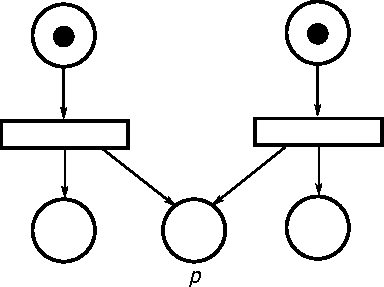
\includegraphics[scale=0.5]{obrazky-figures/PN-parallel2}
		\caption{Ukážka zloženia dvoch sietí. V praxi neužitočné.}
	\end{figure}

	\item Ďaľší prístup je zvážiť ako sa k paralelizmu pristupuje vo výpočetných systémoch. Niekoľko návrhov je schodných. Jeden z najjednoduchších zahŕňa operácie \textbf{FORK} a \textbf{JOIN}. Operácie boli pôvodne navrhnuté Jackom Dennisom a Earlom Van Hornom v roku 1966. Ich prevedenie do Petriho siete je nasledovné: 
	
	\begin{figure}[H]
		\centering
		\begin{minipage}{.4\textwidth}
			\label{fig:fork}
			\centering
			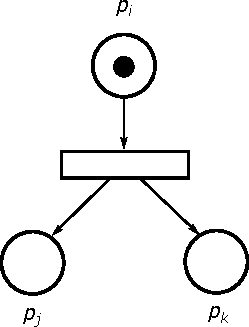
\includegraphics[scale=0.5]{obrazky-figures/PN-fork}
			\caption{Operácia FORK vykonaná v mieste $p_i$ vytvorí proces v miestach $p_j$ a $p_i$.}
		\end{minipage}
	\begin{minipage}{.05\textheight} %spacer
		\quad
	\end{minipage}
		\begin{minipage}{.4\textwidth}
			\label{fig:join}
			\centering
			\includegraphics[scale=0.5]{obrazky-figures/PN-join}
			\caption{Operácia JOIN vykonaná za koncovými miestami procesov $p_j$ a $p_k$ ich spojí a pokračuje v mieste $p_i$.}
		\end{minipage}
	\end{figure}
	
	\item Iný návrh zavedenia paralelizmu je riadiaca štruktúra \textbf{parbegin} a \textbf{parend} [Djikstra 1968]. Koncept navrhnutý Djikstrom má všeobecnú formu $parbegin$ $S_1; S_2;$\dots$S_n$ $parend$, kde $S_i$ predstavuje výraz. Význam $parbegin | parend$ štruktúry je vykonať každý výraz $S_1; S_2;$\dots$S_n$ paralelne. Prevedenie v Petriho sieti je na Obr. \ref{fig:parbegin}.
	
	\begin{figure}[H]
		\centering
		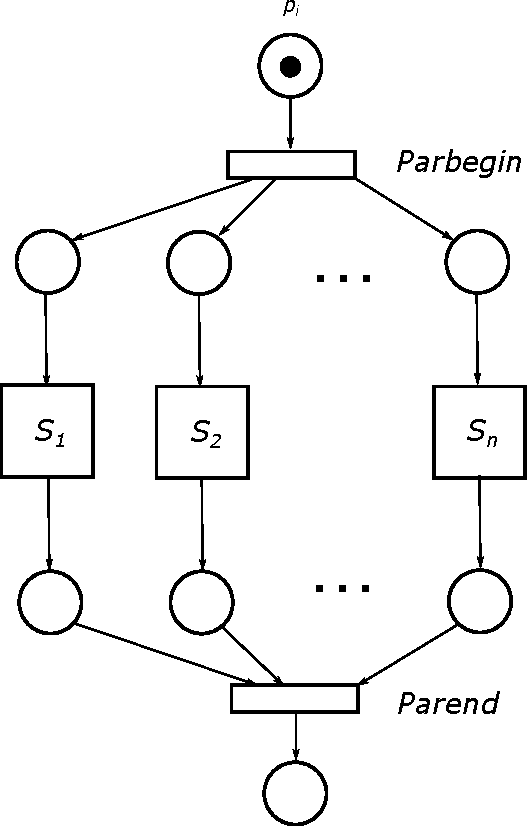
\includegraphics[scale=0.5]{obrazky-figures/PN-parbegin}
		\caption{Riadiaca štruktúra \emph{parbegin} a \emph{parend} v Petriho sieti}
		\label{fig:parbegin}
	\end{figure}
	
	
\end{enumerate} 

\subsection{Čas v Petriho sietiach}

\subsection{Varianty petriho Sietí}
Petriho siete sú koncipované ako plošný (neštrukturovaný) model, kde hierarchický aspekt modelovaného systému nie je nijak vyjadrený. Varianty spomenuté v tejto sekcii sa budú zaoberať rozšírením výpočetnej a modelovacej sily nezbytnej pre prekonanie problému spojeného s plošným statickým modelom. \\\\
\subsubsection{Inhibítory}
Inhibítory umožňujú testovať počet značiek v mieste a tým dávajú Petriho sietiam výpočetnú silu Turingového stroja a sú teda schopné počítať všetky vyčísliteľné funkcie. Takouto sieťou je možné špecifikovat ľubovoľný algoritmus.
\subsubsection{Vysokoúrovňové Petriho siete}
Napriek tomu, že sú siete s inhibítormi schopné vyjadriť akýkoľvek algoritmus, modelovanie čo i len prostého vyhodnocovania aritmetických výrazov je príliš zložité a neintuitívne. Dôvodom sú prostriedky, ktoré zahŕňajú len odjímanie značiek zo vstupných miest a pridávanie značiek do miest výstupných. HL-Siete riešia tento problém zavedením konceptu hranových výrazov, prechodovej stráže a prechodovej akcie.

K tomu, aby sme mohli vysvetliť základné koncepty HL-sítí, potrebujeme pomocný pojem multimnožina a operáciie s multimnožinami.
\begin{defn}
	Majme ľubovolnú neprázdnu množinu $E$. Multimnožina nad množinou $E$ je funkcia. $x : E \longrightarrow \mathbb{N}$. Hodnota $x(e)$ je počet výskytov (koeficient) prvku $e$ v multimnožine $x$. Multimnožinu zapisujeme ako formálnu sumu 
	$$ \sum_{e \in E} x(e)'e $$
	Množinu všetkých multimnožín nad $E$ označíme $E^{MS}$. Pre multimnožiny $x$, $y$ nad $E$ a prirodzené číslo $n$ definujeme:
	
	\begin{enumerate}
		\item sčítanie: $$x + y = \sum_{e \in E} (x(e) + y (e))`e$$
		\item skalárne násobenie: $$n`x = \sum_{e \in E}^{} (n x(e))`e$$
		\item porovnanie:
		$$ x \neq y = \exists e \in E [x(e) \neq y(e) ]$$
		$$ x \leq y = \forall e \in E [x(e) \leq y(e) ]$$
		\item odčítanie: $$x - y = \sum_{e \in E} (x(e) - y (e))`e$$
		\item veľkosť: $$|x| = \sum_{e \in E} x(e)$$
	\end{enumerate}
\end{defn}

\begin{exmpl}
	názorne zápis $2`A + 3`B$ predstavuje multimnožinu s troma výskytmi prvku $a$ a štyrmi výskytmi prvku $b$.
\end{exmpl}

\begin{note}
	Koeficient 1 obvykle vynechávame, tj. napríklad zápis $c$ predstavuje rovnakú multimnožinu ako zápis $1`c$.
\end{note}

Takúto Multimnožinu môžeme konceptom \textbf{hranových výrazov} priradiť k hranám vstupným ako aj výstupným. Názorná ukážka je na Obr. \ref{fig:edge-expr}.

\begin{figure}[H]
	\centering
	\begin{subfigure}[t]{0.4\textwidth}
		\centering
		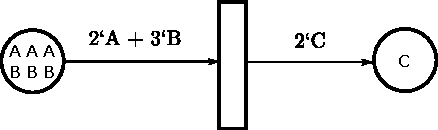
\includegraphics[scale=0.75]{obrazky-figures/PN-edge-expr}
		\caption{Stav pred uskutočnením prechodu}
	\end{subfigure}
	\begin{subfigure}[t]{0.4\textwidth}
		\centering
		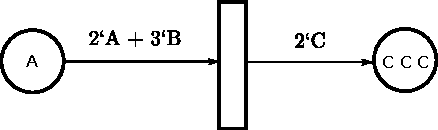
\includegraphics[scale=0.75]{obrazky-figures/PN-edge-exprR}
		\caption{Stav po uskutočnením prechodu}
	\end{subfigure}
	\caption{Hranové výrazy na vstupnej aj výstupnej hrane.}
	\label{fig:edge-expr}
\end{figure}
každému prechodu je možno priradiť \textbf{stráž prechodu}, booleovský výraz, ktorý musí byť splnený pre uskutočnenie prechodu. Je možné určité naviazanie
premenných vo výrazoch na vstupných hranách a rovnako v stráži prechodu. Príklad strážneho výrazu \uv{$x > y$} aj s naväzovaním premenných je na Obr. \ref{fig:guard}.

Pre sugestívnejší zápis dovoluje k stráži prechodu pridať \textbf{akciu prechodu}, odlišujúcu výpočty, ktoré se realizujú pri vykonávaní prechodu, od tých, ktoré se realizujú pri zisťovaní uskutočniteľnosti prechodu.

\begin{figure}[H]
	\centering
	\includegraphics[scale=0.75]{obrazky-figures/PN-guard}
	\caption{Príklad stráže prechodu a akcie prechodu}
	\label{fig:guard}
\end{figure}

\subsubsection{Hierarchické Petriho siete}





\section{PNTalk}

V predošlej kapitole sme sa dozvedeli akú variantu Petriho sietí budeme potrebovať, teraz je na čase predstaviť praktickú implementáciu formalizmu objektovo orientovaných petriho sietí.
\section{Trieda a dedičnosť}

\section{Siete}

\subsection{Objektová sieť}

\subsection{Sieť metód}

\subsection{Sieť konstruktoru}

\subsection{Synchrónny port}

\section{Prechod}

\subsection{Podmienky prechodu}

\subsection{Akcia}

\subsection{Stráž}

\section{PNTalk}

TODO

\chapter{Sekvenčné Diagramy}

Jednou zo štyroch základných modelačných techník UML (Unified Modeling Language) užívanou hojne pri navrhovaní programových systémov je Sekvenčný diagram. Sekvenčný diagram je najbežnejší z kategórie diagramov interakcií a zobrazuje objekty, ktoré sa účastnia v prípade užitia a taktiež zobrazuje správy, ktoré si tieto objekty vymieňajú počas časového intervalu. Diagram je dvojdimenzionálny. Účastníci sú zoradený na horizontálnej ose a časový priebeh je vyjadrený na vertikálnej, kde čas plynie zhora nadol. Ich nespornou výhodou je zobrazovanie aktivity toku správ v časovej postupnosti, to je nápomocné pre porozumenie real-time systémom a komplexným prípadom užitia.

\section{Scenáre}

Sekvenčné diagramy môžu byť generické, zobrazujúce všetky možné scenáre pre definovaný prípad užitia. Častejšie sa však stretneme s vypracovaním diagramov pre jednotlivé scenáre v prípade užitia samostatne.

\section{Komunikácia v sekvenčných diagramoch}

Komunikačný mechanizmus prítomný v sekvenčných diagramoch je, že 
aktivní entity komunikujú priamo, zasielaním správ. 
\begin{note}
	Tu nachádzame konflikt s PT-sieťou v ktorej aktívne entity komunikujú nepriamo, prostredníctvom zdieľaných pasívnych objektov, miestami siete. Mechanizmy sa dajú previesť z jedného na druhý, čo opisuje sekcia :TODO
\end{note}
Sémantika správ je stopa jednoduchej dvojice \lstinline{<sendEvent, RecieveEvent>}, kde \lstinline{sendEvent} je udalosť odoslania správy a \lstinline{recieveEvent} udalosť jej prijatia. Pri absencii jednej udalosti hovoríme o neúplnej správe.

\begin{defn}
	\textbf{Stratená správa} je neúplná správa, pri ktorej je známy výskyt udalosti odoslania správy \lstinline{sendEvent}, ale nie je zaznamenaná udalosť prijatia správy \lstinline{recieveEvent} 
	Typická interpretácia je, že destinácia príjemcu správy je mimo popisovaného rámca. Sémantika je potom zjednodušená na tvar 
	\lstinline{<sendEvent>}.
	Anotácia je šípka vedená od odosielatela zakončená malou bodkou.
\end{defn}

\begin{figure}[H]
	\centering
	\begin{subfigure}[t]{0.4\textwidth}
		\centering
		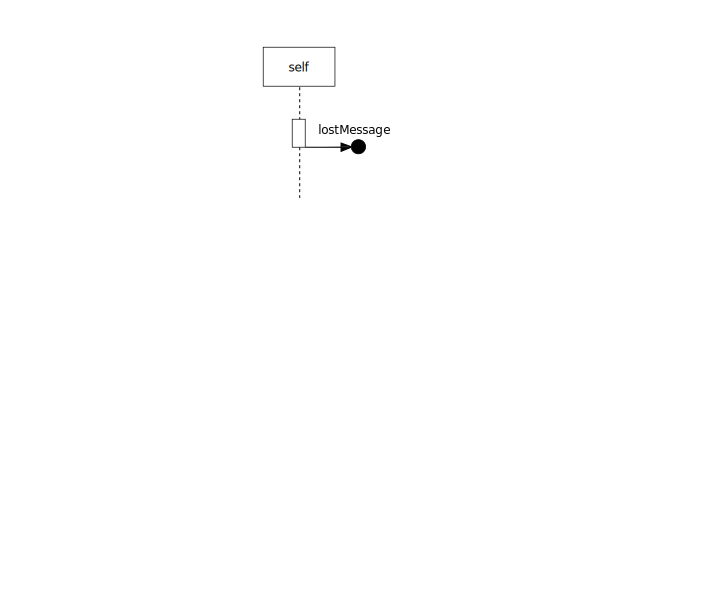
\includegraphics[scale=0.75]{obrazky-figures/SD-lost-ex}
		\caption{Stav pred uskutočnením prechodu}
	\end{subfigure}
	\begin{subfigure}[t]{0.4\textwidth}
		\centering
		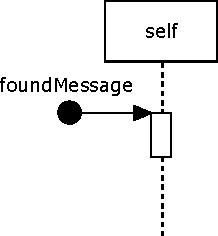
\includegraphics[scale=0.75]{obrazky-figures/SD-found-ex}
		\caption{Stav po uskutočnením prechodu}
	\end{subfigure}
	\caption{Nekompletné správy}
	\label{fig:uncomplete-mes}
\end{figure}

Kompletná správa je v diagrame reprezentovaná orientovanou horizontálnou šípkou smerujúcou od aktívneho objektu odosielateľa k čiare života príjemcu správy. \\\\
V Sekvenčných diagramoch rozlišujeme tri typy správ:

\begin{enumerate}
	\item \textbf{Synchrónna správa} medzi objektami indikuje  sémantiku \emph{wait}, kedy  odosielateľ správy čaká kým je správa spracovaná a pokračuje až po obdržaní odpovede. Správa typicky predstavuje volanie metódy.
	\item \textbf{Asynchrónna správa} používa asynchrónny prístup, pri ktorom nedochádza k žiadnemu blokovaniu objektu odosielateľa. Asynchrónna správa medzi objektami indikuje \emph{no-wait} sémantiku a objekt pokračuje bez toho, aby čakal na odpoveď. Toto dovoľuje paralélne procesy.
	\item \textbf{Odpoveď} predstavuje spätnú správu po synchrónnej správe. Nemôže vzniknúť samostatne.
\end{enumerate}

\begin{figure}[H]
	\centering
	\begin{subfigure}[t]{.3\textwidth}
		\centering
		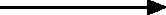
\includegraphics{obrazky-figures/SD-sync}
		\caption{Synchrónna správa}
	\end{subfigure}
	\begin{subfigure}[t]{.3\textwidth}
		\centering
		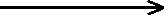
\includegraphics{obrazky-figures/SD-async}
		\caption{Asynchrónna správa}
	\end{subfigure}
\begin{subfigure}[t]{.3\textwidth}
	\centering
	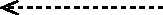
\includegraphics{obrazky-figures/SD-reply}
	\caption{Odpoveď}
\end{subfigure}
	\caption{Reprezentácie troch typov správ}
	\label{fig:arrows}
\end{figure}

\section{Účastníci komunikácie}
Participanti komunikácie skrz správy popísané vyššie sú aktívne objekty, ktoré v sekvenčných diagramoch reprezentujeme čiarou života(\emph{lifeline}).

\begin{defn}
	Pri definícii \textbf{čiary života} začneme netradične notáciou, je zobrazená vertikálnou čiara (môže byť čiarkovaná) predstavujúcu čas života aktívneho objektu. Na jej počiatku sa nachádza hlavička, obdĺžnik obsahujúci \textbf{identifikačnú informáciu} vo formáte: \\
	%\begin{lstlisting}
%<lifelineident> ::= ([<connectable-element-name>[‘[‘ <selector> %‘]’]]
%		[: <connectable-element-type>] [<decomposition>]) | ‘self’
%<selector> ::= <expression>
%<decomposition> ::= ‘ref’ <interactionident> [‘strict’]
%	\end{lstlisting} \vspace{.5cm}
	
	kde \lstinline{<connectable-element-name>} referuje meno typu pripojeného elementu reprezentovaného množinou dodatočných interných datových štruktúr. Napriek tomu, že to zápis dovoľuje \lstinline{<lifelineident>} nemôže byť prázdny.
	
	Ak je identifikátor 'self' čiara života reprezentuje objekt klasifikátoru interakcie, ktorá sama vlastní čiaru života.
	
	
\end{defn} 

\section{Stavebné Elementy sekvenčných Diagramov}

V nasledujúcej sekcii je popísaná syntax a sémantika sekvenčných diagramov.

\subsection{Actor:TODO preklad}

\subsection{objekt}

\subsection{lifeline:TODO preklad čiara života? :D}

\subsection{focus of control:TODO preklad}

\section{Distribuované systémy}

Distribuované systémy majú veľa rozdielnych aspektov, ktoré sa ťažko zachytávajú v jednej difinícii. Je omnoho jednoduchšie hovoriť o distribuovaných systémoch špecifikovaním charakteristík, symptómmi, či média distribúcie. \cite{} V tejto práci budeme mať pod pojmom distribuovaný systém uvažovať systém distribuovaný na počítačovej sieti. \\

Distribúcia prichádza ruka v ruke s vednými disciplínami ako tolerácia chýb, real-time systémy, bezpečnosť a systémový manažment

\subsection{Vymedzenie pojmu distribuovaný systém}

Pred definovaním distribuovaného systému, je vhodné vyjasniť rozdiel s často zameňovaným pojmom počítačových sietí.

\begin{displayquote}
	``Počítačová sieť nie je distribuovaný systém.''
\end{displayquote}

\textbf{Počítačová sieť} je infraštruktúra slúžiaca niekoľkým počítačom  pripojeným k sieti cez komunikačné prepojenie realizované rôznymi médiami a topológiami, a používajú zavedný komunikačný protokol.
Zatiaľ čo \textbf{Distribuovaný systém} je systém pozostávajúci z niekoľkých počítačov, ktoré komunikujú cez počítačovú sieť, hosťujú procesy, ktoré využívajú distribučné protokoly, ktoré zabezpečujú koherentné vykonanie distribuovaných aktivít. \\

\begin{exmpl}
	Vezmime si taký Internet, je to rozsiahla počítačová sieť, vlastne najpodstatnejšia sieť dnes. Používa TCP/IP ako komunikačný protokol.
	Napriek tomu, že tradične poskytuje zopár aplikačných služieb ako e-mail a telnet, nie je to distribuovaný systém. \\
	
	To samozrejme nebráni distribuovaným systémom byť postavených na internete alebo používania internetových technológií, ako distribuované súborové systémy a databázové systémy.
	Jeden z najpodstatnejšįch rozdieľov je, že v prípade distribuovaných systémov procesy zdieľajú spoločný stav a spolupracujú na dosiahnutí spoločného cieľu. Narozdiel od procesov v tomto príklade, ktoré nemusia spolupracovať, len si napríklad vymieňať správy (ako e-mail) bez spoločného cieľu.
\end{exmpl}

\subsection{Porovnanie s Centralizovanými systémami}

V Tabuľke \ref{Tab:central_vs_distr} sú zaznamenané vlastnosti v porovanní s centrálnym systémom ako protipólom k distribuovanému systému. Poznanie rozdieľov, výhod a nevýhod oboch systémov je kľúčové pri návrhu systému. Na základe týchto informácií sa možno ľahšie rozhodnúť, ktorú variantu zvoliť.

\begin{table} [ht]
\begin{center}
	\begin{tabular}{| c | c |} 
		\hline
		Centralizované systémy & Distribuované systémy \\ [0.5ex] 
		\hline\hline
		Dostupnosť & Geografický rámec \\ 
		Homogenita & Heterogenita \\
		Spravovateľnosť & Modularita \\
		 & Škálovateľnosť \\
		 Konzistencia & Zdieľanie \\
		 & Pozvoľná degradácia \\
		 Bezpečnosť & Bezpečnosť \\
		 & Finančný faktor \\ [1ex] 
		\hline
	\end{tabular}
\end{center}
\caption{Porovnanie centralizovaných a distribuovaných systémov}
\label{Tab:central_vs_distr}
\end{table}

Centralizované systémy prirodzene prichádzajú s ľahkou \textbf{dostupnosťou} zdrojov a informácii systému, keďže sú lokálne dostupné. Na druhú stranu Distribuované systémy majú potencionálne \textbf{široký geografický rámec}, preto prístup k zdrojom je niekedy možný len cez vzdialené procedurálne volania.

 \textbf{Homogenita} technológií a procedúr je charakteristická pre centralizované systémy, čím sa myslí jeden operačný systém pre celý systém, ťažké odklonenie sa od používaných technológií systému (programovací jazyk, aplikační rámec). Kdežto u distribuovaných systémov je podporovaná \textbf{heterogenita}, ktorá dovoľuje mať pre každú komponentu odlišné prostredie. Homogenita zjednodušuje správu centrálnych systémov. Heterogenita činí distribuovaný systém inkrementálne rozšíriteľný, ikeď centralizované systémy môžu s dodržaním homogenity dosiahnuť rovnaké rozmery. Skutočná výhoda je až pri \textbf{škálovateľnosti}, kedy centralizované systémy môžu škálovať len \textbf{vertikálne}, to jest zlepšovať výkon nahradzovaním hardvéru za výkonnejší na svojej jednej centrálnej inštancii. Takéto škálovanie je obmedzené technológiou, hardvér sa nedá zlepšovať do nekonečna. Pri distribuovanom systéme máme možnosť škálovať \textbf{horizontálne}, obsluhovať dosiahnutie spoločného cieľu na viacerých inštanciách zároveň. Rozdieľ medzi vertikálnym a horizontálnym škálovaním je graficky znázornený na obrázku \ref{fig:scaling}. 

\begin{figure}[H]
	\centering
	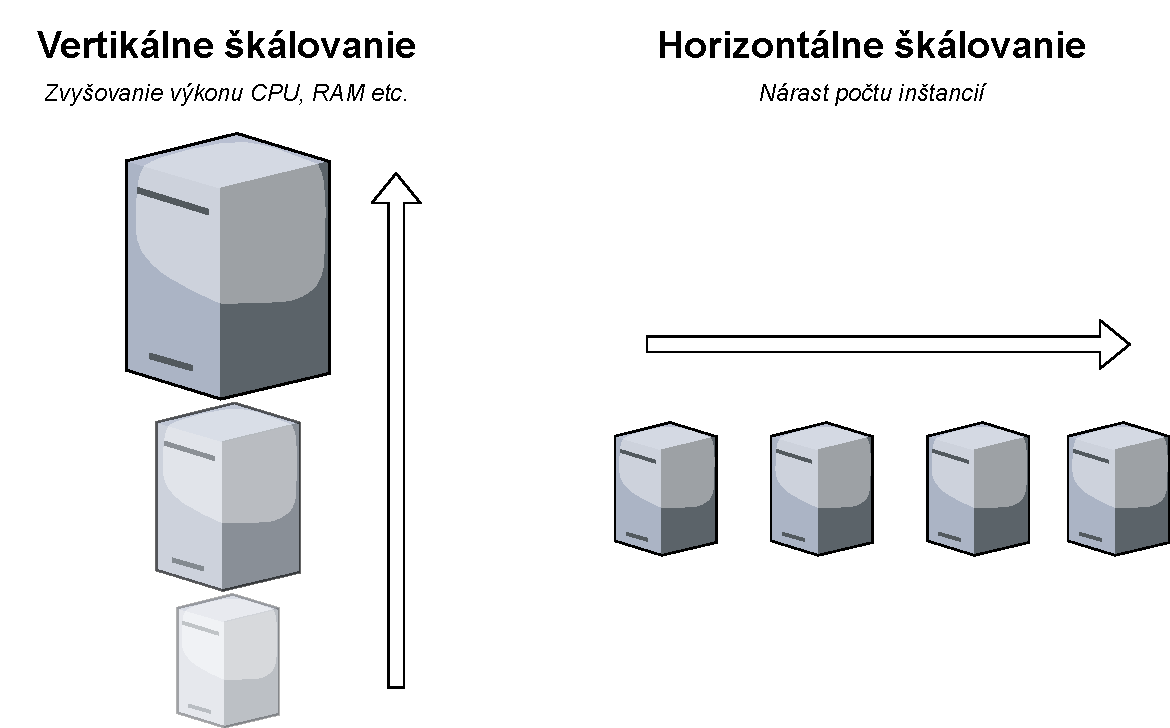
\includegraphics[scale=0.6]{obrazky-figures/TR-scaling}
	\caption{Vertikálne a horizontálne škálovanie}
	\label{fig:scaling}
\end{figure}

\textbf{Konzistenciu} ľahšie dosiahneme u centralizovaných systémov, u distribuovaných je obtiažnejšie zachytiť globálny stav naprieč širokým globálnym rámcom všetkých komponent. \textbf{Pozvoľná degradácia} je vlastnosť systému, ktorý beží kontinuálne spôsobom opatrujúcim možnosť zlyhania komponenty spôsobom, ktorý predíde zlyhaniu celého systému. Tu možno pozorovať silu distribučného systému, kedy pri zlyhaní menšej časti je systém stále dostupný vďaka vysporiadavaniu sa s chybami. Navyše je nepravdepodobné zlyhanie všetkých komponent v rovnaký čas kvôli geografickej separácii jednotlivých komponent.

\textbf{Bezpečnosť} sa dosahuje ľahšie u izolovaného systému s fyzickým prístupom. To nie je možné u distribuovaného systému, avšak vysoká miera bezpečnosti sa dá zaistiť zameraním sa na redukovanie negatívneho efektu vniknutia do systému, než redukovaním hrozieb vzniku neoprávneného vniknutia.

Shrnutím vidíme, že výhody značne prevyšujú ak sa správne rozhodneme, kedy je potreba systém distribuovať.

\subsection{Kedy distribuovať}


Keď nepotrebujeme distribuovaný systém, tak zásadne nedistribujeme. Zbytočne by sme si tým skomplikovali život. Odpoveď pozostáva z troch esenciálnych príčin prečo distribuovať

\begin{enumerate}
	\item Keď má riešený problém decentralizovanú podstatu \\
	\begin{exmpl}
		Zriadujeme systém používajúci konkurenntné procesy na zdrojoch vzdialených pobočiek.
	\end{exmpl}
	\item Keď techniky distribúcie sú vhodnou súčasťou riešenia \\
	\begin{exmpl}
		Systém banky, ktorá potrbuje zálohovať a synchronizovať dáta v dvoch geograficky odľahlých miestach
	\end{exmpl}
	\item Keď problém predpokladá časté zmeny a evolúciu funkcionality, či presunu geografickej polohy. \\
	\begin{exmpl}
		Systém prepožičiavania výpočetných zdrojov medzi vzdialenými uživateľmi.
	\end{exmpl}
\end{enumerate}

\section{Vývojové prostredie}
	Táto kapitola sa zaoberá rozborom vývojových prostredí a ich dekompozíciou na jednotlivé editory a grafické nástroje prítomné v úspešných vývojových prostrediach. \\
	
	Ich význam spočíva v uľahčení práce programátora, zefektívnením kódovania a rýchelho detekovania problémov. Prostredie vedie programátora cez proces editovania, kompilácii či interpretovania kódu a odľaďovania(debugging).
	
	\subsection{Projektový pohľad}
	Predtým než sa pustíme do editovania kódu, musí vývojové prostredie naviazať spojenie s operačným systémom a jeho súborovým systémom. Pri otvorení projektu sken koreňového adresára nahrá do vývojového prostredia kópie súborov a zobrazí ich graficky v projektovom pohľade. Väčšinou je na grafickom uživateľskom rozhraní zobrazovaný pomocou hierarchického stromu, kde listy sú súbory projektu a uzly sú adresáre.
	
	\begin{figure}[H]
		\label{fig:ui-project-pane}
		\centering
		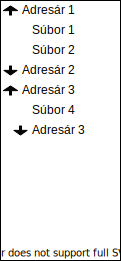
\includegraphics[scale=0.75]{obrazky-figures/UI-project-pane}
		\caption{Ukážka projektového pohľadu s využitím stromovej štruktúry}
	\end{figure}
	
	
	\subsection{Editor zdrojového kódu}
	\label{sec:TR-code-editor}
	Neoddeliteľnou súčasťou každého vývojového prostredia je editor zdrojového kódu, ktorý urýchľuje tvorenie validného kódu v danom programovacom jazyku (väčšina vývojových prostredí má len jeden) za pomoci funkcionalít ako:
	\begin{enumerate}
		\item \textbf{našepkávanie kódu}
		\item \textbf{zvýrazňovanie kľúčových slov}
		\item \textbf{vyhľadávanie a nahradzovanie v kóde}
	\end{enumerate}

	Existuje ich omnoho viac, záleží na konkrétnej implementácii a programovacieho jazyka.
	
	\subsection{Preklad}
	Preklad vo vývojovom prostredí neprebieha na príkazovej riadke, ale odoslanie zdrojových kódov prekladaču alebo interpretu v prípade interpretovaných jazykov je schované v rozhraní za prívetivejšiu variantu tlačítka alebo klávesovej skratky.
	
	\subsection{Ladenie}
	Detekovanie chyby v kóde sa urýchly, ak nám vývojové prostredie umožní kód krokovať, zastaviť a v ktorom koľvek bode sledovať stav premenných.



\chapter{Návrh Implementácie}

Základná myšlienka samotného prevádzania objektovo orientovaných petriho sietí je využiť diskrétnu simuláciu tejto siete, ktorej kroky nám vytvoria časové kontinuum inak chýbajúce v petriho sietiach. 

\section{Architektúra}

Generátor sekvenňých diagramov\cite{Analysis2012} je priamo závislý na dvoch komponentách, validátorom kódu jazyka PNTalk a simulátoru objektovo orientovaných Petriho sietí. Je dôležité zvážiť napojenie týchto komponent ku genrátoru. Vzhľadom k rozličným vlastnostiam jednotlivých implementácii bola motivácia navrhnúť distribuovaný systém s externými komponentami. V generátore uviesť cestu k spustiteľnému binárnemu kódu, ktorého výstup odpovedá definovanému rozhraniu. Daný scenár je uplatniteľný ak pre generátor chceme vyvýjať aj vlastný simulátor, či validátor kódu. V opačnom prípade je vhodnejšie spúšťať externé mikro služby ako webové aplikácie s znovu s vyhradeným komunikačným rozhraním. Pri tejto variante sa namiesto cesty k binárnemu kódu udá generátoru len url adresa webovej aplikace. Tým sa odstráni nechcená závislosť na externej komponente, ktorej pamäťová náročnosť môže presiahnuť pamäťovú náročnosť samotného generátora.

Samotné dáta, prúdiace medzi komponentami, či už vo variante lokálne preloženej binárky, alebo webovej aplikácie musia dodržovať jednotné rozhranie a musia byť serializované zo zrejmých príčin. Pri výbere serializačného formátu je nutno zvážiť viaceré faktory ako podpora v rozličných programovacích jazykoch, ľudsky čiteľnejšie textovo založené formáty alebo binárne uložené dáta, ktoré síce postrádajú ľudskú čiteľnosť no vyžadujú menej pamäte a aj ich zápis a čįtanie je časovo menej náročné. Binárne serializačné formáty by zlepšili responsivitu komponent a dáta posielané v ľudsky čiteľnom formáte by mali nespornú výhodu v odľaďovaní programu. Schodnou variantou sa preto javí podpora viacerých formátov prímaných generátorom od ostatným komponent. Nevýhodou je vznik réžie okolo dohadovaní si serializačného formátu medzi komponentami.

\section{Napojenie na existujúce validátory jazyka PNTalk a simulátory Objektovo orientovaných Petriho sietí}



V tejto Kapitole budú prednesené hlavné myšlienky ako vytvoriť základné stavebné jednotky sekvenčného diagramu. Popisujúc odkiaľ čerpať potrebné informácie zo simulácie, ako si poradiť z neúplnými informáciami a ako sa vysporiadať z absenciou potrebnej informácie zo simulácie OOPN aby bola škoda na výsledku generátora, čo najnižšia. Kapitola je úzko spätá s predchádzajúcimi dvoma kapitolami, keďže bude ťažiť z možností formalismu OOPN a zároveň z vyjadrovacích schopností jazyka PNTalk na vytvorenie datovej štruktúry pre sekvenčný diagram.

\subsection*{Objekt}
Objekt alebo entita je kľúčová časť v scenáry sekvenčného diagramu. Je to obdĺžnik so štítkom mena vo vnútri v ktorom započne čiara života (lifeline) až do deštrukcie objektu, alebo konca simulácie.

\subsubsection*{Vytvorenie objektu}
Na vytvorenie objektu v sekvenčnom diagrame potrebujeme zo simulácie archivovať minimálne 3 veci:

\begin{enumerate}
	\item čas simulácie v ktorom sa inštancia vytvorí
	\item inštanciu, ktorá inicializovala vytvorenie
	\item triedu vytváranej inštancie
\end{enumerate}
Vďaka týmto údajom sa dá vytvoriť správa v sekvenčnom diagrame, ktorá odsadí objekt vertikálne od počiatku do vzdialenosti podľa času vytvorenia.\\\\
\textit{Poznámka: dodatočne sa bude archivovať aj miesto, kam sa objekt uloží pre počítanie referencií. To sa uplatní pri deštrukcii objektu.}


\subsubsection*{Deštrukcia objektu}
Pre deštrukciu objektu musí zaniknúť posledná referencia na objekt. Kvôli tomu je potreba počítadlo referencií, ktoré však nebude výkonnostne náročné ako plnohodnotný garbage collector. Vďaka selektívnemu výberu prechodov, ktoré manipulujú s miestami, kde sú uložené objekty môžme zredukovať počet opakovaní algoritmu len na vybrané prechody.
\pagebreak

Prechod môže spôsobiť tri veci pri manipulácii s referenciou:
\begin{enumerate}
	\item presunúť referenciu do iného miesta\\
	Pri presune referencie sa len pozmení záznam miesta, v ktorom sa nachádza.
	\item zduplikovať referenciu do iného miesta\\
	Pri zduplikovaní sa vytvorí nový záznam o referencii.
	\item vymazať referenciu \\
	Pri vymazaní sa skontroluje, či nie je počet referencií na objekt nulový. Ak áno, objekt sa deštruuje volaním správy destruct z inštancie s prechodom, ktorý poslednú referenciu vymazal.
\end{enumerate}


\subsubsection*{Konvencia mena}

Objekty v sekvenčných diagramoch sa pomenúvavajú pomocou nasledujúcej konvencie "meno inštancie:meno triedy" vďaka čomu môžu vzniknúť tri typy objektov:


\begin{minipage}[c]{0.45\textwidth}
\begin{enumerate}
	\item Pomenovaný objekt
	\item Anonymný objekt
	\item objekt neznámej triedy
\end{enumerate}
\end{minipage}
\hfill
\begin{minipage}[c]{0.8\textwidth}
	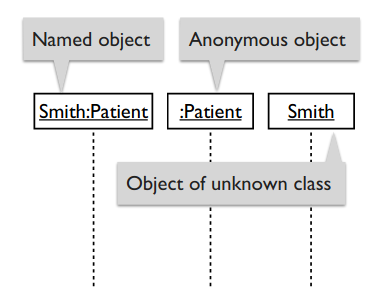
\includegraphics[width=0.45\textwidth]{obrazky-figures/names}
\end{minipage}


syntax jazyka PNTalk vytvára novú inštanciu následovne:

var := classname new.

kde var je dočasná premenná alebo miesto a classname je meno triedy. Problém je zjavný a to, že chýba akákoľvek informácia o mene inštancie. To nám hneď vylúči tretiu možnosť, pretože meno triedy je vždy známe. Varianty sú teda dve a to buď poskladať meno inštancie pomocou známych veličín ako názov miesta, meno triedy, krok simulácie či vygenerovať identifikačné číslo. Druhá varianta je uspokojiť sa s vedomím, že budú vznikať len Anonymné objekty bez názvu inštancie.

\subsection*{Čiara života}
Čiara života alebo inak lifeline je vertikálna čiara reprezentujúca život objektu začína pre každý objekt v dobe vytvorenia a končí deštrukciou objektu, alebo na konci simulácie. Jej vytvorenie je triviálne pokiaľ dokážeme určiť čas vytvorenia a zániku objektu. TODO ref

Je prekrytá bielym obdĺžnikom po dobu, kedy sa metóda objektu nachádza na zásobníku.

\subsubsection*{Na zásobníku}
Doba simulácie po ktorú sa prevádza metóda objektu je viazaná s volaním metód cudzích objektov a preto je nutno archivovať prechody a inštancie, ktoré ich vlastnia. Na tieto prechody potom namapovať prevádzané inštrukcie v chronologickom poradí.

\subsection*{Správa}
Správa vyžaduje poznať odosielateľa, príjemcu a hlavne o aký typ správy sa jedná. Poznáme tri typy:

Synchrónna
Asynchrónna
Odpoveď

zo syntaxe volania metódy pre cudzí objekt evidentne dokážeme zo simulácie odvodiť odosielateľa aj príjemcu.

var methodname: params

kde var je premenná s premennou nesúcou informáciu o mieste s objektom príjemcu. methodname je názov volanej metódy triedy príjemcu. params sú parametre metódy.

odosielateľ je inštancia, ktorá túto akciu zapríčinila svojim prechodom.

Ak metóda vracia hodnotu v simulácii je archivovaná ako odpoveď na správu nesúca údaje o správe na ktorú odpovedá a celú odpoveď.

TODO: Sync vs Async

\subsection*{Cyklus}

K odstráneniu redundantných scenárov značne pomôže zapúzdrenie cyklov, vždy hľadáme v prechodoch najmenší možný ohraničený celok, ktorý sa za sebou sekvenčne niekoľko krát opakuje.

\subsection*{Referovanie a prepájanie diagramov}
Podobne ako pri cykle hľadáme rovnaké, či podobné ohraničené sekvencie prechodov opakujúce sa v simulácii.

\section{Out-source simulácie}

Pre simuláciu bude generátor využívať jeden zo simulátorov objektovo orientovaných petriho sietí z variant bližšie špecifikovaných v kapitole :TODO: . Ako najschodnejšia varianta je zvolený pre túto prácu :TODO: . Aby sme si neuzavreli definitívne dvere k iným implementáciám simulátoru jazyka PNTalk je príhodné zamyslieť sa nad napojením generátoru na simulátor. 

\begin{enumerate}
	\item Varianta pridania kódovej časti do generátoru zjavne možná nie je z dôvodu rôznych implementačných jazykov. Voľba kotlinu ako implementačného jazyka je odôvodnená v sekcii :TODO: .
	
	\item Ponúka sa možnosť vytvoriť dynamickú knižnicu a volať funkcie simulátora z nej. Určite je táto možnosť schodné riešenie, ikeď tu doplácame na neschopnosť preložiť simulátor na všetkých platformách.
	
	\begin{note}
		Linuxová dynamická knižnica *.so nie je ekvivalentná s windowsovou *.dll
	\end{note}
	
	\item Veľmi podobné riešenie je spustiť binárny kód simulátoru s argumentami cestou ku kódu v jazyku PNTalk a zachytením výstupu cout. Oproti predchádzajúcej varianty, vyžaduje omnoho menej úprav.
	
	\item Posledná a taktiež zvolená varianta je pojať generátor ako distribuovaný systém :TODO: , ktorý bude k simulácii využívať komponentu simulátora s ktorou bude komunikovať vopred známym protokolom. To, že si komponenta simulátoru zavolá ďaľšiu komponentu prekladača do medzikódu nebude zo strany generátoru viditeľné. Dôležitý je len pevne daný protokol medzi generátorom a simulátorom, pretože nám to dáva možnosť implementácie simulátoru jednoducho meniť. Stačí aby dodržovali stanovené rozhranie.
	
\end{enumerate}

Distribuovaný systém môže nadobnúť odlišné fyzické formy, či už ide o skupinu osobných počítačov, prepojených lokálnou sieťou, skupinu pracovných staníc zdieľajúcích nielen súborové a databázové systémy, ale navyše aj zdieľaním výpočetnej sily procesora.\cite{}

Distribuovaný systém obsahujúci sadu procesov, ktoré medzi sebou udržujú formu komunikáciu. Okrem konkurenčného behu procesov, niektoré z procesov distribuovaného systému môžu prestať pracovať, pre príklad spadnúť alebo stratiť konektivitu, zatiaľ čo ostatné zostanú bežať a pokračovať v operácii. Toto je podstata čiastočných zlyhaní charakteristických pre distribuované systémy.
\cite{ovilex_ds2016}

\section{Uživateľské rozhranie}

Pri návrhu grafického uživateľského rozhrania je dobré začať položením si otázky "Čo chceme zobrazovať?". Menej je však niekedy viac, pri príliš zložitom rozložení totiž strácame prehľadnosť. \\

\begin{enumerate}
	\item \textbf{Chceme zobraziť momentálne otvorený projekt} \\
	Reprezentáciou by mohol byť hierarchický strom, ktorý by mal v listoch uložené mená súborov a v uzloch mená adresárov. Listy, teda súbory, by mali vizuálnym effektom upozorniť ak je v súbore neuložená zmena. \\
	
	\begin{figure}[H]
		\centering
		\begin{minipage}{.4\textwidth}
			\label{fig:fork}
			\centering
			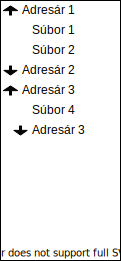
\includegraphics[scale=0.75]{obrazky-figures/UI-project-pane}
			\caption{ Projektový pohľad so schovaným uzlom ``Adresár 2'' a ``Adresár 4''}s
		\end{minipage}
		\begin{minipage}{.05\textheight} %spacer
			\quad
		\end{minipage}
		\begin{minipage}{.4\textwidth}
			\label{fig:join}
			\centering
			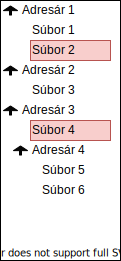
\includegraphics[scale=0.75]{obrazky-figures/UI-project-pane-dirty}
			\caption{Indikácia neuložených zmien v súboroch viditeľná na rozhraní.}
		\end{minipage}
	\end{figure}
	
	\item \textbf{Chceme zobraziť momentálne otvorený súbor s kódom} \\
	Realizujeme to ako editor zdrojového kódu s automatickým zvýrazňovaním kľúčových slov syntaxe jazyka PNTalk a mien z validných definícií. Potrebujeme zobrazovať čísla riadkov.
	\item \textbf{Chceme zobrazovať vygenerovaný diagram} \\
	Potrebujeme na to minimálne rovanko veľa miesta ako na editor zdrojového kódu. Pozadie by malo byť kontrastné vôči diagramu. Celá časť musí byť interaktívna, jednak kvôli pohybu a približovaniu diagramu v okne. Diagram by mal slúžiť ako nástroj na ladenie kódu. To znamená, že kliknutia na jednotlivé časti sekvenčného diagramu by mali vyznačiť reprezentáciu v kóde. Označenie správ by zasa malo zobraziť zmenu miest OOPN, ktoré prechody vyvolali. Označenie, ktoréhokoľvek miesta na čiare života by malo ukázať aktuálne hodnoty v miestach danej inštancie.
	\item \textbf{Chceme zobrazovať posledných \textit{x} riadkov logov}
	Je fajn dať uživateľovi vedieť čo sa deje formou správ, či už chybových alebo informačných. Správy sa musia dať kopírovať a musia byť viditeľné od najnovšej po najstaršiu.
	\item \textbf{Chceme zbytok funkcionalít ukryť do hornej lišty}
	V hornej lište by mali byť kategoricky roztriedené funkcie, s klávesovými skratkami u tých, u ktorých to dáva zmysel.
\end{enumerate}

\subsection{Rozloženie uživateľského rozhrania}

Nie je treba znovu vynaliezať koleso. Pri návrhu rozloženia elementov uživateľského rozhrania sa preto budeme inšpirovať úspešnými vývojovými prostrediami (Visual Studio, IntelliJ IDEA).
To samozrejme neplatí o netradičnom elemente vykresľujúci sekvenčný diagram, je to časť ktorá zobrazuje výstup a zároveň je to aj interaktívny debugger. Inšpiráciu pre tento element by sme hľadali márne, v bežných vývojových prostrediach sa nič podobné nenachádza.
Ničmenej je rovnako, ak nie viac, dôležitý ako editor zdrojového kódu, preto dostane rovnako veľké miesto. \\

Po zvážení veškerých nárokov na uživateľské rohranie vyšlo z procesu návrhu rozloženie na obr. :TODO:

\begin{figure}[H]
	\label{fig:ui-layout}
	\centering
	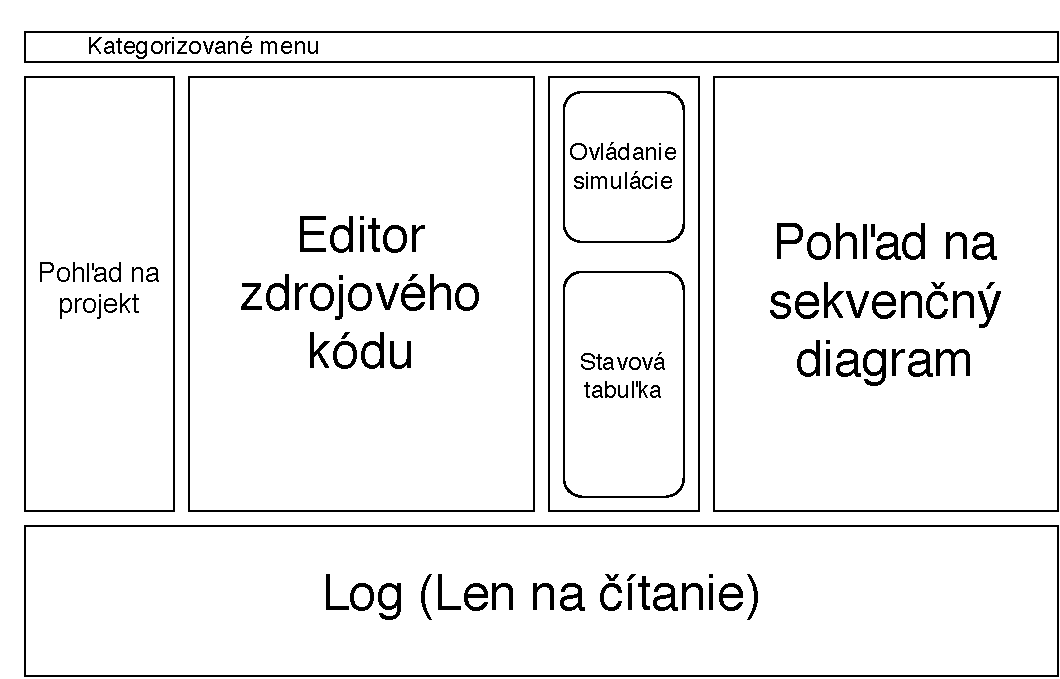
\includegraphics[scale=0.75]{obrazky-figures/UI-layout}
	\caption{Návrh rozloženia grafického uživateľského rozhrania}
\end{figure}



\chapter{Implementácia}

\section{Implementácie distribuovaného systému pomocou Dockeru}

Ako bolo zmienené v návrhu, 

\section{Uživateľské rozhranie}

Implementácia vychádza z dobre pripraveného návrhu v sekcii :TODO: , ktorá bola realizovaná za pomoci kotlinovského aplikačného rámcu TornadoFX nad softvérovou platformou JavaFX.

\subsection{JavaFX v kotline} 

\subsection{Editor Zdrojového kódu}

V sekcii \ref{sec:TR-code-editor} boli vymenované niektoré funkcionality, ktoré nesmú chýbať v moderných editoroch zdrojového kódu. Z nich bolo implementované zvýrazňovanie kľúčových slov jazyka PNtalk a zvýrazňovanie všetkých validne definovaných názvov tried, prechodov, miest, synchrónnych portov a metód.

Zvýrazňovanie zaisťuje asynchrónna funkcia computeHighlighting volaná nad textom z editoru. Je postavená na vyhľadávaní regulárnych výrazov. Globálne v celom rámci sa zvýrazňujú kľúčové slová jazyka PNTalk a mená tried. V rámci danej triedy sa k nim pridá vyhľadávanie názvov prechodov, miest, synchrónnych portov definovaných však len v rozsahu danej triedy.

\chapter{Záver}

Práca demonštroje automatický prevod objektovo orientovaných Petriho sietí na sekvenčné diagramy, generovanie však pokrýva len podmnožinu sekvenčných diagramov. Objekty Actors vystupujúce v konvenčne vytvorených sekvenčných diagramoch sú v práci zanedbané (keďže informáciu na rozlíšenie obyčajných objektov od Actors nedokázali poskytnúť definície v kóde, ani následná simulácia) a Actors preto vystupujú len ako všeobecné objekty. Ďaľší zrejmý nedostatok vyplýva z naviazania na neúplnú implementáciu simulátora, ktorá neumožňuje simuláciu všetkých validných konštrukcií jazyka PNTalk, len ich podmnožinu. Istou kompenzáciou jest architektúra navrhnutá ako distrubovaný systém, ktorá robí tento problém ľahko riešiteľným v budúcnosti po implementovaní vhodnejšej varianty simulátora. Na Záver je vhodné položiť si otázku či sme boli úspešný.
To nám zodpovie sada validačných testov. Jedná sa o netriviálne Petriho siete zadefinované v jazyku PNTalk, ktorých vygenerované výstupy boli porovnané s tými ručne vytvorenýmí. Okrem validity vzišla motivácia zaznamenať výsledky aj časovej náročnosti. Časová náročnosť sa merala pre samotný proces generácie sekvenčných diagramov ako aj celkovo beh v spolupráci externých komponent. Plán bol vytýčiť hranice, pre ktoré by bolo reálne simulovať a vykreslovať výsledok generácie ihneď pri zmene vstupnęho kódu. Kvôli neuspokojivým výsledkom v tomto teste (:TODO: graf) sa z pokusu o implementácie funkcie "hot-reload" upustilo. 

\section{Výsledky testovania}




 


  \fi
  
  % Kompilace po částech (viz výše, nutno odkomentovat)
  % Compilation piecewise (see above, it is necessary to uncomment it)
  %\subfile{projekt-01-uvod-introduction}
  % ...
  %\subfile{chapters/projekt-05-conclusion}


  % Pouzita literatura / Bibliography
  % ----------------------------------------------
\ifslovak
  \makeatletter
  \def\@openbib@code{\addcontentsline{toc}{chapter}{Literatúra}}
  \makeatother
  \bibliographystyle{bib-styles/Pysny/skplain}
\else
  \ifczech
    \makeatletter
    \def\@openbib@code{\addcontentsline{toc}{chapter}{Literatura}}
    \makeatother
    \bibliographystyle{bib-styles/Pysny/czplain}
  \else 
    \makeatletter
    \def\@openbib@code{\addcontentsline{toc}{chapter}{Bibliography}}
    \makeatother
    \bibliographystyle{bib-styles/Pysny/enplain}
  %  \bibliographystyle{alpha}
  \fi
\fi
  \begin{flushleft}
  \bibliography{literatura-bibliography}
  \end{flushleft}

  % vynechani stranky v oboustrannem rezimu
  % Skip the page in the two-sided mode
  \iftwoside
    \cleardoublepage
  \fi

  % Prilohy / Appendices
  % ---------------------------------------------
  \appendix
\ifczech
  \renewcommand{\appendixpagename}{Přílohy}
  \renewcommand{\appendixtocname}{Přílohy}
  \renewcommand{\appendixname}{Příloha}
\fi
\ifslovak
  \renewcommand{\appendixpagename}{Prílohy}
  \renewcommand{\appendixtocname}{Prílohy}
  \renewcommand{\appendixname}{Príloha}
\fi
%  \appendixpage

% vynechani stranky v oboustrannem rezimu
% Skip the page in the two-sided mode
%\iftwoside
%  \cleardoublepage
%\fi
  
\ifslovak
%  \section*{Zoznam príloh}
%  \addcontentsline{toc}{section}{Zoznam príloh}
\else
  \ifczech
%    \section*{Seznam příloh}
%    \addcontentsline{toc}{section}{Seznam příloh}
  \else
%    \section*{List of Appendices}
%    \addcontentsline{toc}{section}{List of Appendices}
  \fi
\fi
  \startcontents[chapters]
  \setlength{\parskip}{0pt} 
  % seznam příloh / list of appendices
  % \printcontents[chapters]{l}{0}{\setcounter{tocdepth}{2}}
  
  \ifODSAZ
    \setlength{\parskip}{0.5\bigskipamount}
  \else
    \setlength{\parskip}{0pt}
  \fi
  
  % vynechani stranky v oboustrannem rezimu
  \iftwoside
    \cleardoublepage
  \fi
  
  % Přílohy / Appendices
  \ifenglish
    \input{projekt-30-prilohy-appendices-en}
  \else
    \chapter{Obsah přiloženého paměťového média}

\chapter{Manuál}

  \fi
  
  % Kompilace po částech (viz výše, nutno odkomentovat)
  % Compilation piecewise (see above, it is necessary to uncomment it)
  %\subfile{projekt-30-prilohy-appendices}
  
\end{document}
